\documentclass{astroedu-lab}
\usepackage{graphicx}
\usepackage{subcaption}

\begin{document}

\pagestyle{plain}

\begin{problem}{\huge Лабораторная работа 5.4.1\\\\Определение теплоты испарения\\\\жидкости\\\\Выполнил Жданов Елисей Б01-205}

\section{Цель работы}

Измерить пробег $\alpha$-частиц в воздухе двумя способами: с помощью торцевого счетчика Гейгера и синтиляционного счетчика, -- по полученным данным определить энергию частиц.

\section{Теоретическая часть}
	При $\alpha$-распаде исходное родительское ядро испускает ядро гелия и превращается в дочернее ядро, число протонов и число протонов уменьшается на две единицы. Функциональная свзяь между энергией $\alpha$-частицы $E$ и периодом полураспада радиоактивного ядра $T_{1/2}$ хорошо описывается формулой
	\begin{equation*}
		 \lg T_{1/2} = \frac{a}{\sqrt{E}} + b.
	\end{equation*}
	Экспоненциальный характер этого процесса возникает вследствие экспоненциального затухания волновой функции в области под барьером, где потенциальная энергия больше энергии частицы.
	
	Для описания связи между энергией $\alpha$-частицы и ее пробегом пользуются эмпирическими соотношениями. В диапазоне энергий $\alpha$-частиц от 4 до 9 МэВ эта связь хорошо описывается выражением
	\begin{equation*}
		\label{eq:R(E)}
		\tag{$\star$}
		R = 0,32E^{3/2}
	\end{equation*}

\section{Экспериментальная установка}
	В данной работе пробег $\alpha$-частиц в воздухе определяется треями способами:

		
\begin{figure}[h!]
    \centering
    \begin{subfigure}{0.3\textwidth}
        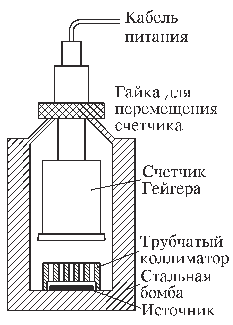
\includegraphics[scale=1]{ustanovka1.pdf}
        \caption{Счетчик Гейгера}
        \label{pic1}
    \end{subfigure}
    \begin{subfigure}{0.3\textwidth}
        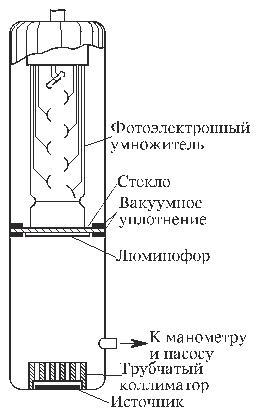
\includegraphics[scale=0.8]{ustanovka2.pdf}
        \caption{Сцинциллятор}
        \label{pic2}
    \end{subfigure}
    \begin{subfigure}{0.3\textwidth}
        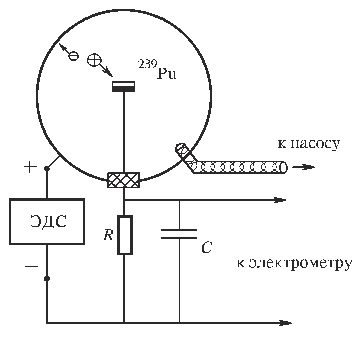
\includegraphics[scale=1]{ustanovka3.pdf}
        \caption{Ионизационная камера}
        \label{pic3}
    \end{subfigure}
    \caption{Экспериментальные установки.}
    \label{fig:ustanovki}
\end{figure}

	
	В качестве источника $\alpha$-частиц используется ${239}$Pu с периодом полураспада $T_{1/2} = 2,44 \cdot 10^4$ лет. Альфа-частицы, испускаемые ${239}$Pu состоят их трех моноэнергетических групп, различие между которыми лежит в пределах 50 кэВ. При той точности, которая достигается в наших опытах, их можно считать совпадающими по энергии, равной 5,15 МэВ.
	

%
%Найдем угловые коэффициенты прямых для каждой установки по МНК.
%
%\[
%	a = \frac{<x_i y_i> - < x > < y_i >}{< x_i^2> - < x_i >^2}
%\]
%
%\[
%	b = < \nu_i > - a < N_i >
%\]
%
%Также рассчитаем их погрешности
%
%\begin{equation}
%	S_a^2 = \frac{< x_i^2>}{< x_i^2 > - < x_i >^2} \cdot \frac{<  b_i - b > ^2}{n - 2}
%\end{equation}


%\begin{center}
%	\Large $q(T)$
%\end{center}

%\begin{figure}[!h]
%	\centering
%	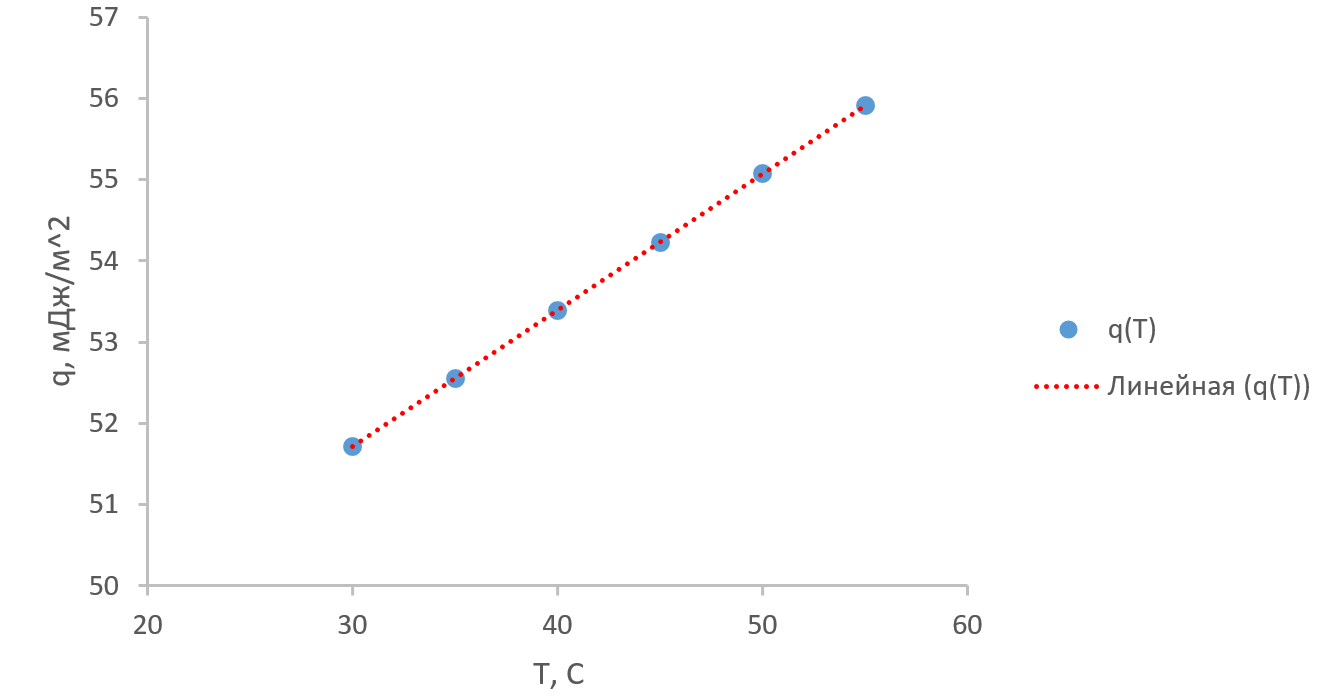
\includegraphics[width=1\textwidth]{2023-02-23_22-23-59.png}
%	\label{fig:boiler}
%\end{figure}

\section{Обработка результатов}
		\subsection{Исследование пробега $\alpha$-ч. счетчика Гейгера}	
		Представим результаты измерений (табл.) зависимости $N=N(x)$ в виде графика -- рис. 
		
		\begin{figure}[h!]
		\centering
			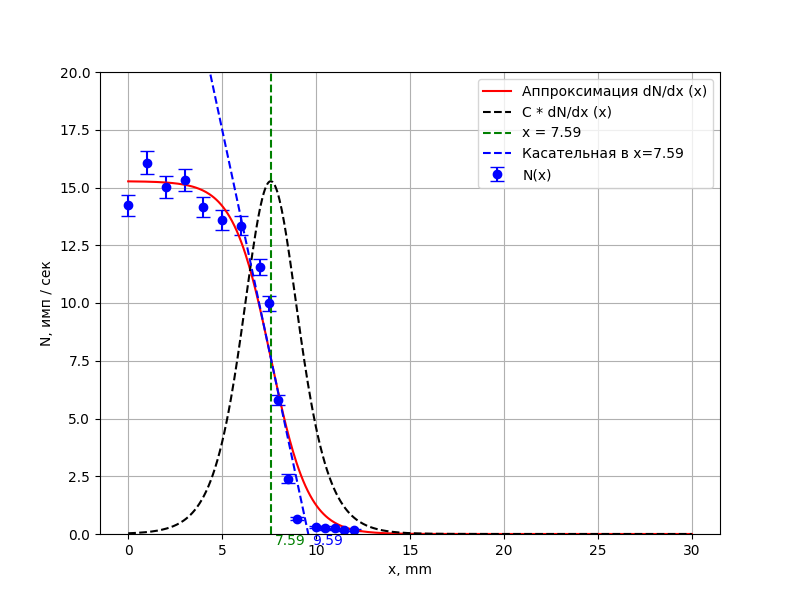
\includegraphics[scale=0.5]{Figure_1.png}
		\end{figure}
	
		Найдем кривую, приближающую экспериментальные точки, в следующем виде:
		\begin{equation*}
			N (x) = \frac{A}{1+e^{(x-x_0)/dx}}.
		\end{equation*}
		
Аппроксимация сигмоидой, причем значение на $+\infty$ было выбрано строго 0, чтобы избежать нереалистичного (отрицательного) сдвига отсчетов при больших расстояниях x.
	
	
		\begin{table}[H]
			\caption{Параметры аппроксимации.}
			\label{tab:pfrfmetry1}
			\centering
			\begin{tabular}{|c|c|c|}
				\hline
				$A_1$ & $x_0$, мм & $dx$, мм \\ \hline
				15.3 & 7.6   & 0.6           \\ \hline
			\end{tabular}
		\end{table}
		
Погрешность x было решено взять среднему расстоянию от кривой до точек графика на отвесной части графика.
	
		Средний $R_\text{ср}$ и экстраполированный $R_\text{экстр}$ пробеги определяются следующими уравнениями:
		\begin{equation*}
			\begin{cases}
				N^{\prime \prime} (R_\text{ср}) = 0, \\
				R_\text{экстр} = R_\text{ср} + \left|N(R_\text{ср})/N^\prime(R_\text{ср})\right|.
			\end{cases}
		\end{equation*}
	
		Энергию можно найти из формулы : $E = \left(R/0,32\right)^{2/3}$.
	\\
			\begin{table}[h!]
			\centering
				{\begin{tabular}{|c|c|}
						\hline
						$R_\text{ср}$, см & $R_\text{экстр}$, см \\ \hline
						$1.76 \pm 0.06 $   & $1.96 \pm 0.08$       \\ \hline
				\end{tabular}}
				\\.\\.\\
				{\begin{tabular}{|c|c|}
						\hline
						$E(R_\text{ср})$, МэВ & $E(R_\text{экстр})$, МэВ \\ \hline
						$3.12 \pm 0.08 $     & $3.35 \pm 0.10 $        \\ \hline
				\end{tabular}}     
		\end{table}
	
	
		\newpage
		\subsection{Исследование пробега $\alpha$-ч. с помощью сцинтилляционного счетчика}	
		Представим результаты измерений (табл.) зависимости $N=N(P)$ в виде графика -- рис. 
		
		\begin{figure}[h!]
		\centering
		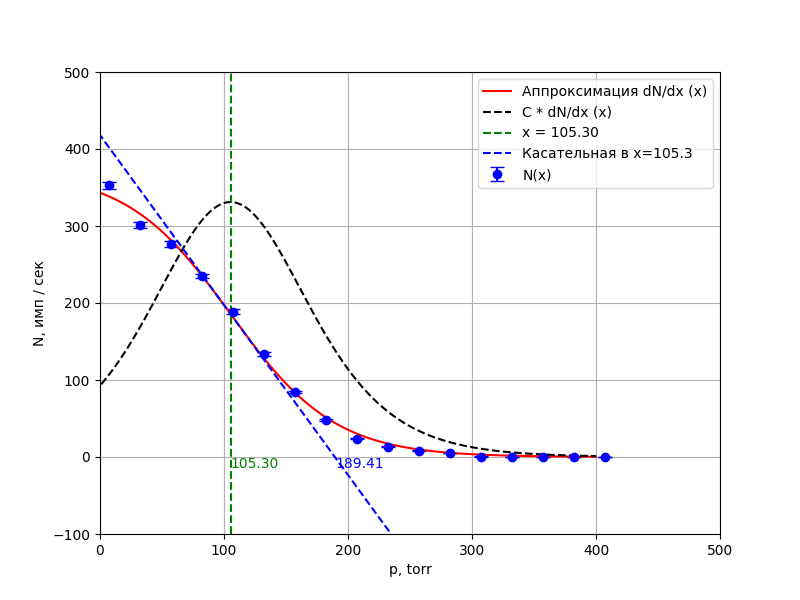
\includegraphics[scale=0.5]{Figure_2.png}  
		\end{figure}
		
		Найдем кривую, приближающую экспериментальные точки, в следующем виде:
		\begin{equation*}
			N (P) = \frac{A}{1+e^{(P-P_0)/dp}}.
		\end{equation*}
		
		\begin{table}[H]
			\caption{Параметры аппроксимации.}
			\label{tab:parametry2}
			\centering
			\begin{tabular}{|c|c|}
				\hline
				$A$ & $P_0$, торр \\ \hline
				$371$  & $110 \pm 50$      \\ \hline
			\end{tabular}
		\end{table}
		
		Давления $P_\text{ср}$ и $P_\text{экстр}$, которые соответсвуют среднему $R_\text{ср}$ и экстраполированному $R_\text{экстр}$ пробегам, очевидно, определяются следующей системой уравнений:
		\begin{equation*}
			\begin{cases}
				N^{\prime \prime} (P_\text{ср}) = 0, \\
				P_\text{экстр} = P_\text{ср} + \left|N(P_\text{ср})/N^\prime(P_\text{ср})\right|.
			\end{cases}
		\end{equation*}
	
		\begin{table}[H]
			\caption{P.}
			\label{tab:P}
			\centering
			\begin{tabular}{|c|c|}
				\hline
				$P_\text{ср}$, торр & $P_\text{экстр}$, торр \\ \hline
				$105 \pm 15 $   & $190 \pm 20$       \\ \hline
			\end{tabular}
		\end{table}
	
		\newpage
		Так как $\alpha$-частицы не могут достигнуть люминофора при обычном давлении, то свободный пробег будет равен расстоянию между препаратом и люминофором -- 9 см. Следовательно, мы можем пересчитать средний и экстраполированные свободные пробеги частиц к давлению 760 торр и температуре 15$^\circ$:
		\begin{equation*}
			R = \frac{288 \ \text{К}}{T} \cdot \frac{P}{760 \ \text{торр}} \cdot 9 \ \text{см}.
		\end{equation*}
		
		\begin{table}[h!]
		\centering
		\begin{tabular}{|c|c|}
						\hline
						$R_\text{ср}$, см & $R_\text{экстр}$, см \\ \hline
						$1.3 \pm 0.6 $   & $2.2 \pm 0.2$       \\ \hline
				\end{tabular}
				{\begin{tabular}{|c|c|}
						\hline
						$E(R_\text{ср})$, МэВ & $E(R_\text{экстр})$, МэВ \\ \hline
						$2.6 \pm 0.7 $     & $3.6 \pm 0.2 $        \\ \hline
				\end{tabular}}   
		\end{table}
	
		\subsection{Определение пробега $\alpha$-ч. с помощью ионизационной камеры}
			Представим результаты измерений (табл.) зависимости $I=I(P)$ в виде графика -- рис. 
		
		\begin{figure}[h!]
		\centering
		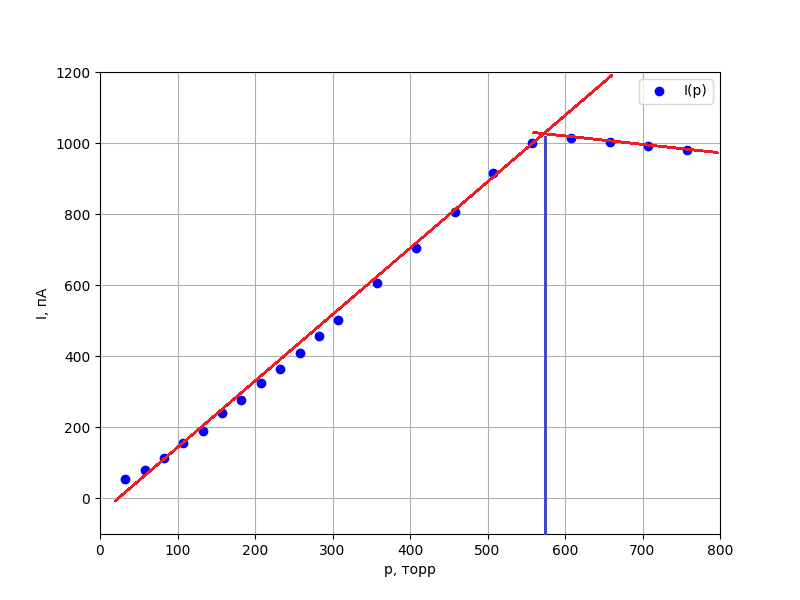
\includegraphics[scale=0.5]{Figure_3.png}  
		\end{figure}
		
		По графику определим: $P_\text{экстр} = (570 \pm 10)$ торр(с использованием кусочного МНК). Аналогично предыдущему пункту найдём экстраполированный пробег $R_\text{экстр}$ и соответствующую энергию.
		\begin{equation*}
			R = \frac{288 \ \text{К}}{T}\frac{P}{760 \ \text{торр}}\, \frac{10 - 0.5}{2} \ \text{см},
		\end{equation*}
		где 0.5 см и 10 см -- диаметры первого и второго электродов соответственно.
		\begin{table}[h!]
		\centering
				\begin{tabular}{|c|}
						\hline
						$R_\text{экстр}$, см $\ \ \ $ \\ \hline
						$3.44 \pm 0.07$         \\ \hline
				\end{tabular}
				\begin{tabular}{|c|}
						\hline
						$E(R_\text{экстр})$, МэВ \\ \hline
						$4.87 \pm 0.07 $            \\ \hline
				\end{tabular}      
		\end{table}
\newpage
\section{Обсуждение результатов и выводы}
	В работе тремя различными способами был измерен свободный пробег в воздухе $\alpha$-частиц  с энергией 5.15 МэВ. В качестве источника радиоактивных частиц был использован $^{239}$Pu.
	
Величины энергий ядер гелия измеренных Гейгером: 3.35 МэВ; сцинциллятором 3.6 МэВ; ионизационной камерой 4.87 МэВ. В пределах возможных случайных и систематических погрешностей значения совпадают с энергией частиц, но все числа систематически ниже ожидаемого значения.
	
	Результаты вычислений энергий для экстраполированных и средних пробегов (см. таблицы) по эмпирической формуле ($R = 0.32E^{3/2}$) привели к заниженным значениям. Это может быть следствием угловой расходимости пучка $\alpha$-частиц. Экспериментально наблюдаемые зависимости числа $\alpha$-частиц от глубины их проникновения качественно правильно передают провявление брэгговского пика и, тем самым, относительную величину пробега частиц с разной энергией. Однако в силу указанных причин брэгговский пик оказывается смещенным и сильно размытым. Поэтому экстраполированный пробег дает лучшую оценку.

Также поскольку источник частиц покрыт слюдяной пленкой, что может происходить замедление $\alpha$-частиц. Эмпирическая формула энергии в области энергий 4-5.5 МэВ требует уточнений. Свободный пробег (выраженный в г/см$^2$) слюдяной пленки несколько больше свободного пробега в воздухе, выраженного в тех же единицах.
	
%	Для уточнения формулы~(\ref{eq:R(E)}) вычислим по ней значения энергий для известных длин свободного пробега в воздухе и найдем разницу -- таблица~\ref{table:conclusion}. Видно, что в диапазоне от 1,58 до 5,58 имеется наибольшее расхождение\footnote{вблизи нуля тоже, но в данной работе эта область нас не интересует}. Поэтому найдем степенную функцию, которая лучше всего в среднем квадратичном приближает табличные значения в интересующем нас диапазоне. Имеем:
%	\begin{equation}
%		\tag{$\star \star$}
%		E = a\,R^{b},
%	\end{equation}
%	где $a$ и $b$ -- постоянные, значения которых приведены рис.~\ref{fig:conclusion}.
%	


%Если плотность бумаги равна $ 1.2 \text{г}/\text{см}^3 $,
%следовательно, лист бумаги толщины $l\geq~R'/\rho = 36.6 $
%мкм не пропустит альфа-частицы от $ ^{239}  $Pu.

	
%
%
%	\begin{figure}[h!]
%	\centering
%	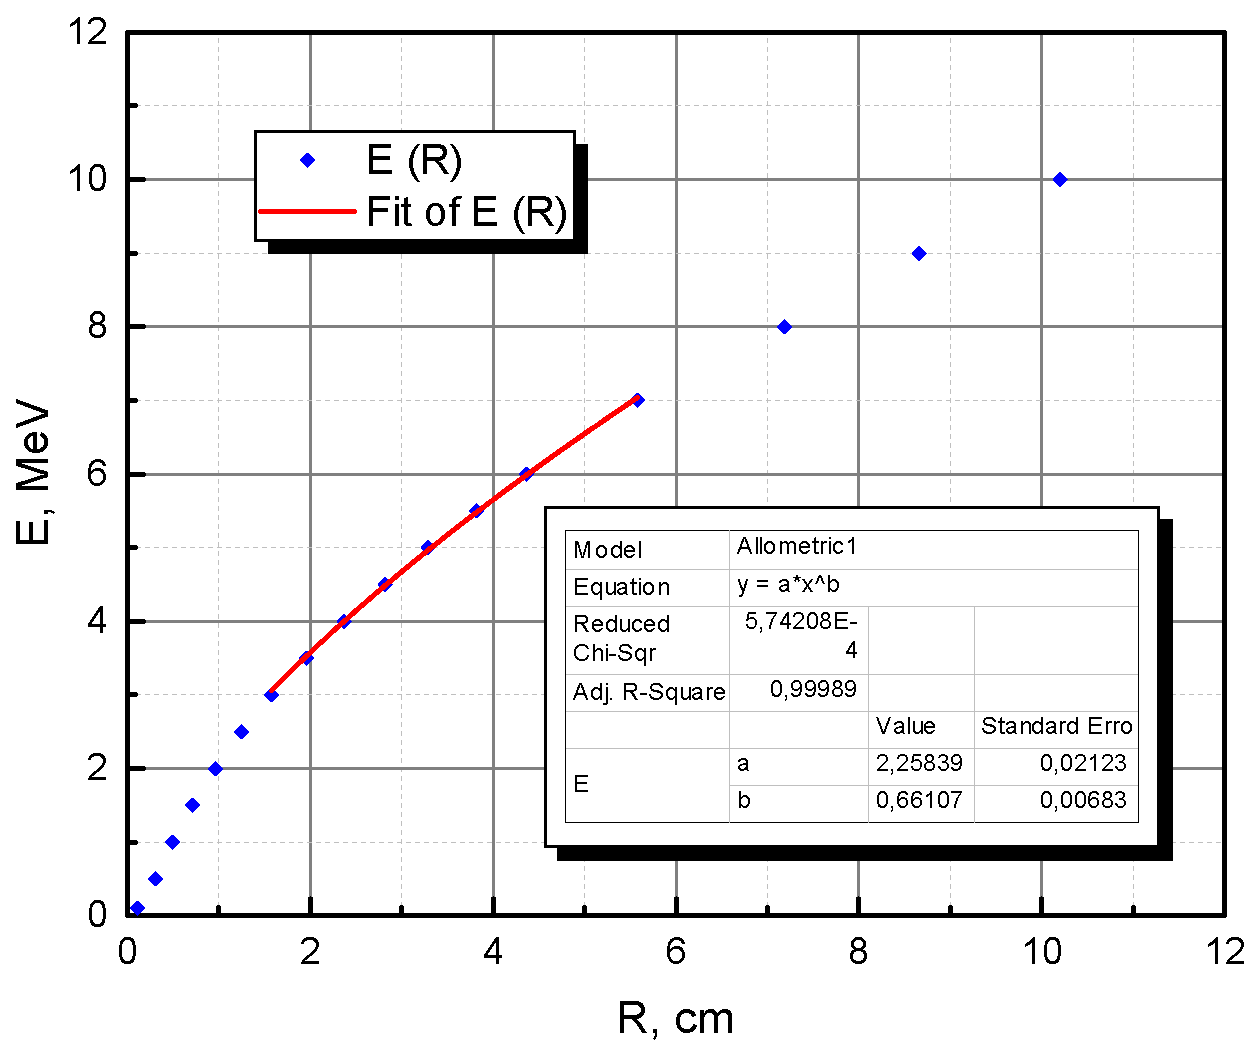
\includegraphics[scale=0.5]{graph4.pdf}
%	\end{figure}


\section{Ресурсы}

Расчет по МНК: метод-наименьших-квадратов.рф


\end{problem}
\end{document}